\documentclass{beamer}
\usetheme{metropolis}

\usetheme{metropolis}

\usepackage[ngerman]{babel}
\usepackage[autostyle=true,german=quotes]{csquotes}
\usepackage[linewidth=1pt]{mdframed}
\usepackage{hyperref}
\usepackage{makecell}
\usepackage{pifont}
\usepackage{tikz}
\usetikzlibrary{positioning, calc, arrows, fit, decorations.pathreplacing, shapes, shapes.multipart, snakes}
\usepackage{verbatim}
\usepackage{textcomp}
\usepackage{centernot}
\usepackage{tabularx}
\usepackage{ulem}
%\usepackage{pdfpages}

\batchmode

\hypersetup{
	colorlinks,
	urlcolor=blue,
	linkcolor=black % for ToC
}
\newenvironment{qaa}[1]{
	#1

	\begin{mdframed}
		\small
}{
	\end{mdframed}
}

\newcommand{\true}{\ding{51}}
\newcommand{\false}{\ding{55}}
\newcommand{\code}[1]{
	\begin{mdframed}
		\verbatiminput{#1}
	\end{mdframed}
}


\title{Tutorium 03: Typen und Typklassen}
% \subtitle{}
\author{Paul Brinkmeier}
\institute{Tutorium Programmierparadigmen am KIT}
\date{09. November 2020}

\begin{document}

\begin{frame}
	\titlepage
\end{frame}

\section{Heutiges Programm}
\begin{frame}{Programm}
	\begin{itemize}
        \item Übungsblätter 1 und 2
		\item Wiederholung der Vorlesung: Typen und Typklassen
		\item Datentypen selbst definieren
	\end{itemize}
\end{frame}

\section{Übungsblatt 1}

\begin{frame}{1.2.\{1,2\} -- Insertionsort}
  \code{../demos/InsertSort.hs}
\end{frame}

\begin{frame}{1.2.\{3,4\} -- Mergesort}
  \code{../demos/MergeSort.hs}
\end{frame}

\section{Übungsblatt 2}

\begin{frame}{2.1 -- Bindung und Gültigkeitsbereiche}
    \begin{figure}
        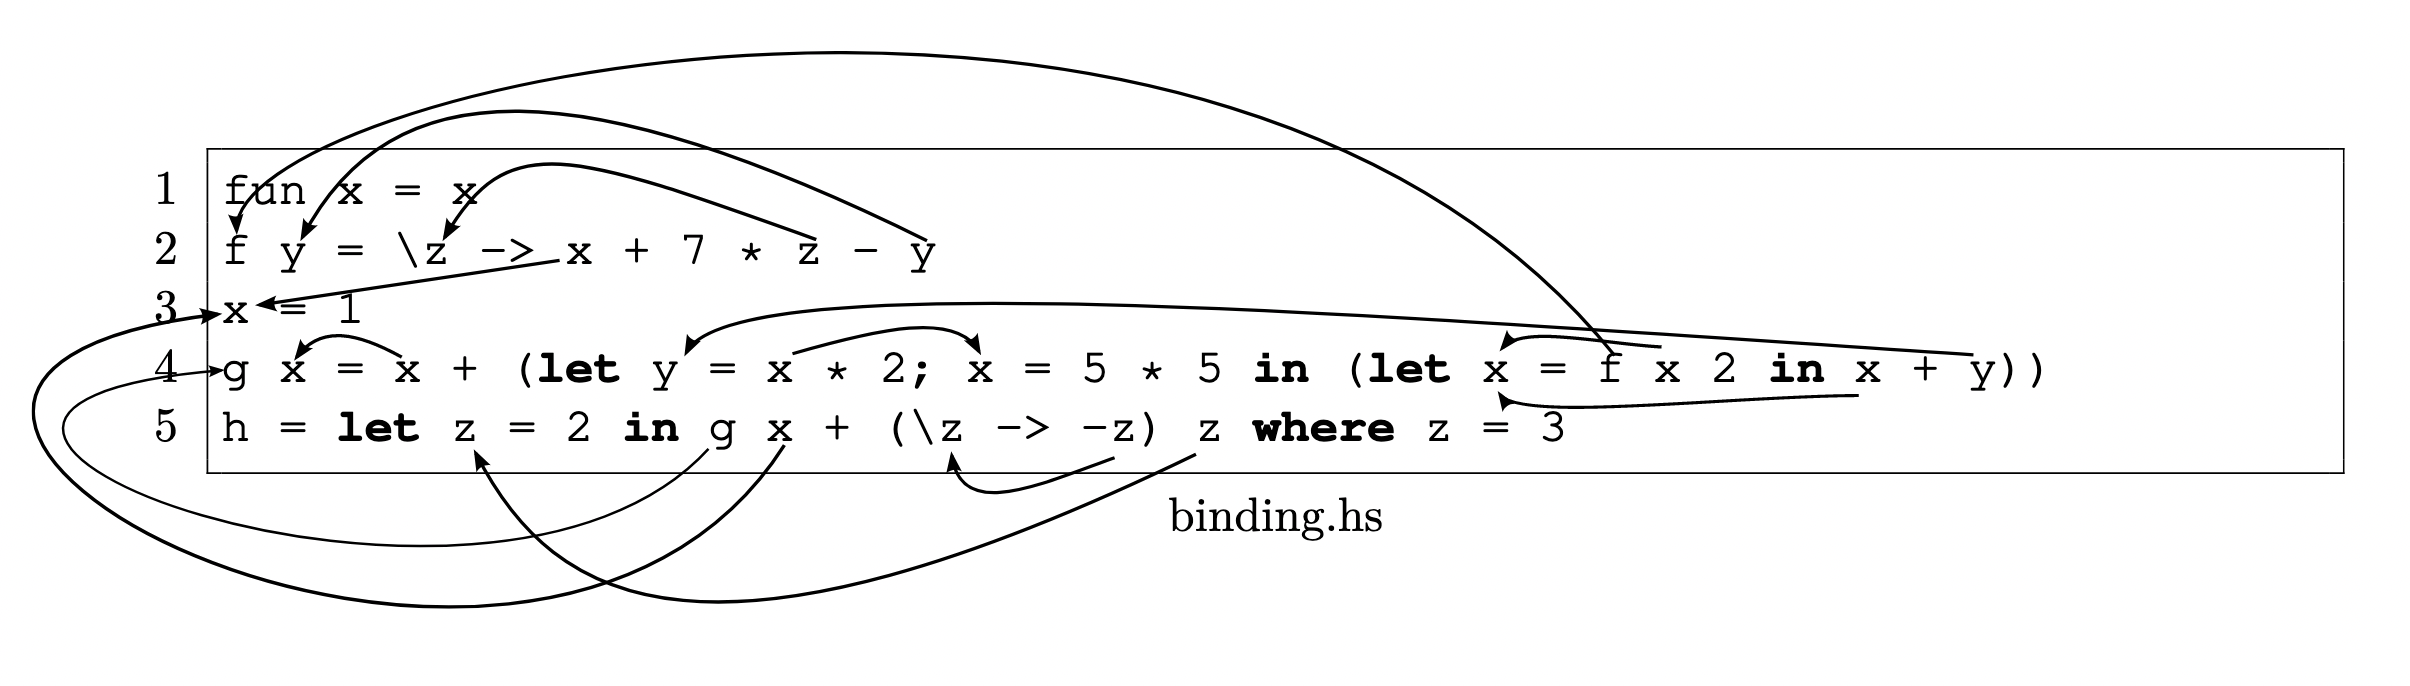
\includegraphics[width=\textwidth]{images/binding.png}
    \end{figure}

    \begin{itemize}
        \item Größte Fehlerquelle: \texttt{x * 2} und \texttt{f x 2} in Zeile 4
        \item Beide zeigen auf Definition im selben \texttt{let}-Block
        \item $\leadsto$ Allgemein: Variablen zeigen möglicherweise auf eine Definition im selben \texttt{let}-Block, selbst wenn es ihre eigene ist.
    \end{itemize}
\end{frame}

\begin{frame}{2.2.\{1,2,3\} -- Polynome}
  \code{../demos/Polynom.hs}

  \texttt{(\$) :: (a -> b) -> a -> b} -- Funktionsanwendung als Operator.
\end{frame}

\section{Wiederholung:\\Typen und Typklassen}

\begin{frame}{Cheatsheet: Typen}
  \begin{itemize}
    \item \texttt{Char}, \texttt{Int}, \texttt{Integer}, ...
    \item \texttt{String}
    \item \emph{Typvariablen}/\emph{Polymorphe Typen}:
    \begin{itemize}
      \item \texttt{(a, b)}: Tupel
      \item \texttt{[a]}: Listen
      \item \texttt{a -> b}: Funktionen
      \item Vgl. Java: \texttt{List<A>}, \texttt{Function<A, B>}
    \end{itemize}
    \item \emph{Typsynonyme}: \texttt{type String = [Char]}
  \end{itemize}
\end{frame}

\begin{frame}{Cheatsheet: Algebraische Datentypen in Haskell}
  \begin{itemize}
    \item \emph{\texttt{data}-Definitionen}, \emph{Datenkonstruktoren}
    \item Algebraische Datentypen: \emph{Produkttypen} und \emph{Summentypen}
    \begin{itemize}
      \item Produkttypen $\approx$ \texttt{struct}s in C
      \item Summentypen $\approx$ \texttt{enum}s
    \end{itemize}
    \item \emph{Typkonstruktoren}, bspw. \texttt{[] :: * -> *}
    \item \emph{Polymorphe} Datentypen, bspw. \texttt{[a]}, \texttt{Maybe a}
    \item Beispiel:
  \end{itemize}
  \code{../demos/Shape.hs}
\end{frame}

\begin{frame}{Cheatsheet: Typklassen 1}
  \begin{itemize}
    \item \emph{Klasse}, \emph{Operationen}/\emph{Methoden}, \emph{Instanzen}
    \item Beispiele:
    \begin{itemize}
      \item \texttt{Eq t}, $\{ \texttt{(==)}, \texttt{(/=)} \}$, $\{ \texttt{Eq Bool}, \texttt{Eq Int}, \texttt{Eq Char}, ... \}$
      \item \texttt{Show t}, $\{ \texttt{show} \}$, $\{ \texttt{Show Bool}, \texttt{Show Int}, \texttt{Show Char}, ... \}$
    \end{itemize}
    \item Weitere Typklassen: \texttt{Ord}, \texttt{Num}, \texttt{Enum}
    \item Deklaration/Implementierung:
  \end{itemize}

  \code{../demos/Truthy.hs}
\end{frame}

\begin{frame}{Cheatsheet: Typklassen 2}
  \begin{itemize}
    \item \emph{Vererbung}: Typklassen mit Voraussetzungen
  \end{itemize}

  \code{../demos/Truthy2.hs}
\end{frame}

\section{Typen selbst definieren}

\begin{frame}{Typen selbst definieren}
  Modelliert mit \texttt{data}:

  \vfill

  \begin{itemize}
    \item Führerschein
    \item Spielkarten
    \item Monopolykarten
    \item Boolesche Ausdrücke
    \item (Typen in Haskell)
    \item MiMa-Instruktionen
  \end{itemize}

  \vfill

  Vorlagen: \href{https://codi.pbrinkmeier.de/s/wq88qbGYy}{codi.pbrinkmeier.de/s/wq88qbGYy}
\end{frame}

\begin{frame}{Führerschein}
  \code{../demos/DriversLicense.hs}

  \vfill

  \begin{itemize}
    \item Klasse B kann Zusatzziffer B96 haben.
    \item Für Daten gibt es natürlich auch eigene Typen.
    \item Beispiel:\\
          \texttt{DriversLicense [A, B True] "{}Arthur"{} (1, 1, 1970)}
  \end{itemize}
\end{frame}

\begin{frame}{Spielkarten}
  \code{../demos/PlayingCard.hs}
\end{frame}

\begin{frame}{Monopolykarten}
  \code{../demos/Monopoly.hs}
\end{frame}

\begin{frame}{Boolesche Logik}
  \code{../demos/BoolExpr.hs}

  \vfill

  Beispiele:
  \begin{itemize}
    \item $a \wedge b$ entspricht \texttt{BinaryOp (Var "{}a"{}) AND (Var "{}b"{})}
    \item $a \vee (b \wedge 0)$ entspricht\\
          \texttt{BinaryOp (Var "{}a"{}) AND (BinaryOp (Var "{}b"{}) OR (Const False))}
  \end{itemize}
\end{frame}

\begin{frame}{MiMa}
  \code{../demos/MiMa.hs}
\end{frame}

\section{Typklassen implementieren}

\begin{frame}{Implementierung von Typklassen}
  Implementiert:

  \vfill

  \begin{itemize}
    \item Monopolykarten: \texttt{Eq MonopolyCard}, \texttt{Show MonopolyCard}
    \item Boolesche Ausdrücke: \texttt{Show BoolExpr}
    \item Typen in Haskell: \texttt{Show Type}
    \item MiMa-Instruktionen: \texttt{Show MiMaInst}
    \item Spielkarten: \texttt{Eq} und \texttt{Ord} für \texttt{Suit}, \texttt{Rank} und \texttt{PlayingCard}
    \begin{itemize}
      \item \texttt{Ord PlayingCard}: Zuerst nach Farbe, dann nach Wert.
    \end{itemize}
  \end{itemize}

  \vfill
  
  Aufgabe: Spielkarten + eine weitere
\end{frame}

\begin{frame}{\texttt{Ord PlayingCard} -- Vorlage}
  \code{../demos/PlayingCard2.hs}
\end{frame}

\begin{frame}{\texttt{Ord PlayingCard} -- Automatische Instanz durch \texttt{deriving}}
  \code{../demos/PlayingCard3.hs}

  \texttt{Enum} ermöglicht es, bspw. \texttt{[Hearts .. Spades]} zu schreiben.
\end{frame}

\end{document}
